
A DC amplifier has an open loop gain of 1000 and two poles, a dominant one at 1kHz and a high frequency one whose location can be controlled. It is required to connect this amplifier in a negative feedback loop that provides a DC closed loop gain of 10 and a maximally flat response. 

\begin{enumerate}[label=\arabic*.,ref=\theenumi]
%\begin{enumerate}[label=\thesubsection.\arabic*.,ref=\thesubsection.\theenumi]
\numberwithin{equation}{enumi}
%\numberwithin{figure}{enumi}

\item Find the required value of $H$.
\\
\solution Table \ref{table:ee18btech11005_ Input_Table} summarises the given information.  The open loop gain can be expressed as
\begin{align}
\label{eq:ee18btech11005_open_loop_gain} 
  G(s) &= \frac{G_0}{\brak{1+\frac{s}{p_{1}}}\brak{1+\frac{s}{p_{2}}}} 
\\
\implies G(0) &= G_0
\end{align}
The closed loop gain 
\begin{align}
 \label{eq:ee18btech11005_transfer_function}
    T(s) &= \frac{G(s)}{1+G(s)H}
\\
\implies T(0) &= \frac{G_0}{1+G_0H}
\end{align}
%
Substituting from Table \ref{table:ee18btech11005_ Input_Table}, 
%But,also given DC closed loop gain is 10. DC closed loop gain is given in equation.\ref{eq:ee18btech11005_dc_gain} 
\begin{align}
\frac{1000}{1+1000H} &= 10
\\
\implies H &=  0.099 
\label{eq:ee18btech11005_h_value}
\end{align}
%
\begin{table}[!ht]
\centering
\input{./tables/ee18btech11005/ee18btech11005_1.tex}
\caption{1}
\label{table:ee18btech11005_ Input_Table}
\end{table}
\begin{align}
    G_0 &= 1000\\
\text{Therefore.,} G(s)&= \frac{1000}{(1+\frac{s}{p_{1}})(1+\frac{s}{p_{2}})}  
\end{align}
%Let, -p1 be the dominant pole.
%\begin{align}
%    p_1 &= 2\pi10^3 rad/sec
%\end{align}
%Now, we connect the system in a negative feedback of feedback factor H.
%------------------------------
\item Find $p_2$.
\\
\solution From \eqref{eq:ee18btech11005_transfer_function} and \eqref{eq:ee18btech11005_open_loop_gain},
\begin{align}
%    T(s) &= \frac{\frac{G_0}{(1+\frac{s}{p_{1}})(1+\frac{s}{p_{2}})}}{1+\frac{HG_0}{(1+\frac{s}{p_{1}})(1+\frac{s}{p_{2}})}}\\
%    T(s) &= \frac{\frac{p_1p_2G_0}{(p_1+s)(p_2+s)}}{1+\frac{p_1p_2HG_0}{(p_1+s)(p_2+s)}}
%\end{align}
%\begin{align}
%    T(s) &= \frac{p_1p_2G_0}{(p_1+s)(p_2+s) + p_1p_2HG_0}\\
%    T(s) &= \frac{p_1p_2G_0}{p_1p_2+(p_1+p_2)s+s^2 + p_1p_2HG_0}\\
    T(s) &= \frac{p_1p_2G_0}{s^2+(p_1+p_2)s+(HG_0+1)p_1p_2} \label{eq:ee18btech11005_closed_loop}
\\
&= \frac{K \omega_n^{2}}{s^2+2\zeta\omega_ns+\omega_n^{2}}
\\
%\label{eq:ee18btech11005_second_order_ce}
\implies 
\begin{split}
    \omega_n &= \sqrt{(HG_0+1)p_1p_2}\\
    \zeta &= \frac{p_1+p_2}{2\sqrt{(HG_0+1)p_1p_2}}
\end{split}
\label{eq:ee18btech11005_second_order_zeta}
\end{align}
using the standard formulation for a second order system.  Also, for maximally flat response, the quality factor 
%Q of equation.\ref{eq:ee18btech11005_second_order_ce}, is given by
\begin{align}
    Q = \frac{1}{2\zeta}= \frac{1}{\sqrt{2}}&
\\
\implies  \zeta = \frac{1}{\sqrt{2}} &
\label{eq:ee18btech11005_second_order_zeta_q}
\\
\implies \frac{p_1+p_2}{2\sqrt{(HG_0+1)p_1p_2}} &= \frac{1}{\sqrt{2}}
%\end{align}
\\
%\begin{multline}
\implies \sqrt{\frac{p_1}{p_2}}+\sqrt{\frac{p_2}{p_1}} 
%\\
&= \sqrt{2(HG_0+1)} 
\end{align}
%\end{multline}
%
The above equation is of the form 
%
\begin{align}
\label{eq:ee18btech11005_x}
x + \frac{1}{x} &= a
\\
\implies x &= \frac{a \pm \sqrt{a^2 -4}}{2}
\label{eq:ee18btech11005_x_sol}
\end{align}
%
where 
\begin{align}
\label{eq:ee18btech11005_x_p1p2}
x  &= \sqrt{\frac{p_2}{p_1}}
\\
a &= \sqrt{2(HG_0+1)}, 
\label{eq:ee18btech11005_a}
\end{align}
Thus, from \eqref{eq:ee18btech11005_x_p1p2}, \eqref{eq:ee18btech11005_a}
and \eqref{eq:ee18btech11005_x_sol},
%
\begin{align}
p_2 &= p_1\sbrak{\frac{\sqrt{2\brak{HG_0+1}} \pm \sqrt{2 \brak{HG_0+1}-4}}{2}}^2
\end{align}
%
From the following code,
\begin{lstlisting}
codes/ee18btech11005/ee18btech11005_1.py
\end{lstlisting}
%
\begin{multline}
p_2 = 1244038.9567529503 
\\
\text{ and } 31.734068607786863
\end{multline}
%
%---------------------
\item  Draw the equivalent circuit system diagram.\\
\solution
The equivalent circuit system is shown in the figure.\ref{fig:equivalent_system}
\begin{figure}[!hbt]
	\begin{center}
			\resizebox{\columnwidth}{!}{\input{./figs/ee18btech11005/equivalent_control_system.tex}}
	\end{center}
\caption{1}
\label{fig:equivalent_system}
\end{figure}
%-----------------
\item Obtain $G(s)$ and $T(s)$
\\
\solution Substituting the value of $p_2$ in  \eqref{eq:ee18btech11005_open_loop_gain} and \eqref{eq:ee18btech11005_closed_loop},
\begin{align}
     G(s) &= \frac{1000}{(1+\frac{s}{2\pi10^3})(1+\frac{s}{1.244\times10^6})}
    \label{eq:ee18btech11005_G(s)}
\\
    T(s) &= \frac{10}{0.128\times10^{-11}s^2+1.599\times10^{-6}s+1}
    \label{eq:ee18btech11005_Transfer_func}
\end{align}
%--------------------------

\item Verify from the Bode plot of above closed loop transfer function that it has maximally flat response.
\\
\solution The following code generates the bode plot of the transfer function in Fig. \ref{fig:ee18btech11005_1}.
\begin{lstlisting}
codes/ee18btech11005/ee18btech11005_2.py
\end{lstlisting}
\begin{figure}[!ht]
\centering
\includegraphics[width=\columnwidth]{./figs/ee18btech11005/ee18btech11005_1.eps}
\caption{}
\label{fig:ee18btech11005_1}
\end{figure}
%---------------------------------
\item Find the step response of $T(s)$
\\
\solution The following code generates the desired response of in Fig. \ref{fig:ee18btech11005_2}.
\begin{lstlisting}
codes/ee18btech11005/ee18btech11005_3.py
\end{lstlisting}
%
\begin{figure}[!ht]
\centering
\includegraphics[width=\columnwidth]{./figs/ee18btech11005/ee18btech11005_2.eps}
\caption{}
\label{fig:ee18btech11005_2}
\end{figure}

%-------------------------------
\item Design a circuit that represents the above transfer function.\\
\solution The circuit can be designed using  operational amplifiers having negative feedback.Consider the circuit shown in figure.\ref{fig:circuit_design}:1.Assume the gain of all the amplifiers are large.And assume no zero state response.Take the parameters in s-domain.\\
\begin{figure}[!hbt]
	\begin{center}
			\resizebox{\columnwidth}{!}{\begin{circuitikz}
\ctikzset{bipoles/length=1cm}

\draw 
(0, 0) node[op amp] (opamp) {$1$}
(4.5, -0.35) node[op amp] (opamp2) {$2$}
(opamp.-) -- (-1,0.35) -- (-1.5,0.35) to[R=$R_1$] (-3,0.35){}
(-1,0.35)-- (-1,1) to[C=$C_1$] (1.5,1) -- (1.5,0){}
(1.5,0)--(2,0) to[R=$R_2$] (3,0)--(3.5,0)--(opamp2.-){}
(opamp2.+)--(3.5,-0.7) node[ground]{}
(opamp.out)--(1.5,0){}
(opamp.+) -- (-1.5,-0.35) -- (-1.5,-1.5) 
(6,-1.5) to[C=$C$] (6,-3) node[ground]{}
(-1.5,-1.5) to[R=$R$] (6,-1.5) --(6,-0.35){}
(3.5,0) -- (3.5,0.75)--(4,0.75) to[C=$C_2$] (6,0.75) -- (6,-0.35){}
(opamp2.out) -- (6,-0.35){}
(6,-0.35)--(6.5,-0.35)
node at (-1,0.2){A}
node at (3.5,-0.2){B}
node at (1.5,-0.4){$V_1$}
node at (6.3,-0.6){$V_{out}$}
node at(-3,0.7){$V_{in}$}
node at(-1,-0.6){$V_1^1$}
node at (6.7,-1.5){$C$}
;\end{circuitikz}

}
	\end{center}
\caption{1}
\label{fig:circuit_design}
\end{figure}
\textbf{For the first amplifier,}\\
\begin{align}
    \frac{V_{in}-V_1^1}{R_1} &= \frac{V_1^1-V_1}{\frac{1}{sC_1}}\\
    \frac{V_{in}}{R_1} &= \frac{V_1^1}{R_1}+sC_1V_1^1 - sC_1V_1 \\
    \frac{V_{in}}{R_1} &= V_1^1\sbrak{sC_1+\frac{1}{R_1}}-sC_1V_1\\
    V_{in} &= V_1^1(sC_1R_1+1)-sC_1R_1V_1\label{eq:opamp_1}
\end{align}
\textbf{For the second amplifier.,}
\begin{align}
    \frac{V_1-V_b}{R_2} &= (V_b-V_{out})sC_2\\
    \text{Since.,} V_b &= 0\\
    \implies V_1 &= -sC_2R_2V{out}\label{eq:opamp2}
\end{align}
\textbf{Voltage division at node C.,}\\
\begin{align}
    \frac{V_1^1}{V_{out}} &= \frac{1+\frac{1}{sC}}{\frac{1}{sC}}\\
    \implies V_1^1 &= (sCR+1)V_{out}\label{eq:Voltage_division}
\end{align}
From eq:\eqref{eq:opamp_1} ,eq:\eqref{eq:opamp2} ,eq:\eqref{eq:Voltage_division}
\begin{align}
     V_{in} = ((sCR+1)(sC_1R_1+1)+s^2C_1R_1C_2R_2)V_{out}\\
\end{align}
 \begin{multline}
   \frac{V_{in}}{V_{out}}=s^2(CRC_1R_1+C_1R_1C_2R_2) + s(CR+C_1R_1) + 1\\
   \frac{V_{out}}{V_{in}}=\frac{1}{s^2(CRC_1R_1+C_1R_1C_2R_2) + s(CR+C_1R_1) + 1} \label{eq:Circuit_trans_func}
\end{multline}
Comparing the equation.\eqref{eq:ee18btech11005_Transfer_func} and equation.\eqref{eq:Circuit_trans_func}\\
\begin{align}
      C_1R_1(CR+C_2R_2) &= 0.128\times10^{-11} \\
   CR+C_1R_1 &= 1.599\times10^{-6}\\
  \text{Let.,} CR&= 10^{-6}\\
  \implies C_1R_1 &= 0.599\times 10^{-6}\\
  0.599\times 10^{-6}(10^{-6}+C_2R_2) &= 0.128\times10^{-11}\\
  C_2R_2 &= 0.681\times10^{-6}
\end{align}
The parameters can be chosen as shown in the TABLE:\ref{table:ee18btech11005_ Output_Table}\\
\begin{table}[!ht]
\centering

%%%%%%%%%%%%%%%%%%%%%%%%%%%%%%%%%%%%%%%%%%%%%%%%%%%%%%%%%%%%%%%%%%%%%%
%%                                                                  %%
%%  This is the header of a LaTeX2e file exported from Gnumeric.    %%
%%                                                                  %%
%%  This file can be compiled as it stands or included in another   %%
%%  LaTeX document. The table is based on the longtable package so  %%
%%  the longtable options (headers, footers...) can be set in the   %%
%%  preamble section below (see PRAMBLE).                           %%
%%                                                                  %%
%%  To include the file in another, the following two lines must be %%
%%  in the including file:                                          %%
%%        \def\inputGnumericTable{}                                 %%
%%  at the beginning of the file and:                               %%
%%        \input{name-of-this-file.tex}                             %%
%%  where the table is to be placed. Note also that the including   %%
%%  file must use the following packages for the table to be        %%
%%  rendered correctly:                                             %%
%%    \usepackage[latin1]{inputenc}                                 %%
%%    \usepackage{color}                                            %%
%%    \usepackage{array}                                            %%
%%    \usepackage{longtable}                                        %%
%%    \usepackage{calc}                                             %%
%%    \usepackage{multirow}                                         %%
%%    \usepackage{hhline}                                           %%
%%    \usepackage{ifthen}                                           %%
%%  optionally (for landscape tables embedded in another document): %%
%%    \usepackage{lscape}                                           %%
%%                                                                  %%
%%%%%%%%%%%%%%%%%%%%%%%%%%%%%%%%%%%%%%%%%%%%%%%%%%%%%%%%%%%%%%%%%%%%%%



%%  This section checks if we are begin input into another file or  %%
%%  the file will be compiled alone. First use a macro taken from   %%
%%  the TeXbook ex 7.7 (suggestion of Han-Wen Nienhuys).            %%
\def\ifundefined#1{\expandafter\ifx\csname#1\endcsname\relax}


%%  Check for the \def token for inputed files. If it is not        %%
%%  defined, the file will be processed as a standalone and the     %%
%%  preamble will be used.                                          %%
\ifundefined{inputGnumericTable}

%%  We must be able to close or not the document at the end.        %%
	\def\gnumericTableEnd{\end{document}}


%%%%%%%%%%%%%%%%%%%%%%%%%%%%%%%%%%%%%%%%%%%%%%%%%%%%%%%%%%%%%%%%%%%%%%
%%                                                                  %%
%%  This is the PREAMBLE. Change these values to get the right      %%
%%  paper size and other niceties.                                  %%
%%                                                                  %%
%%%%%%%%%%%%%%%%%%%%%%%%%%%%%%%%%%%%%%%%%%%%%%%%%%%%%%%%%%%%%%%%%%%%%%

	\documentclass[12pt%
			  %,landscape%
                    ]{report}
       \usepackage[latin1]{inputenc}
       \usepackage{fullpage}
       \usepackage{color}
       \usepackage{array}
       \usepackage{longtable}
       \usepackage{calc}
       \usepackage{multirow}
       \usepackage{hhline}
       \usepackage{ifthen}



%%  End of the preamble for the standalone. The next section is for %%
%%  documents which are included into other LaTeX2e files.          %%
\else

%%  We are not a stand alone document. For a regular table, we will %%
%%  have no preamble and only define the closing to mean nothing.   %%
    \def\gnumericTableEnd{}

%%  If we want landscape mode in an embedded document, comment out  %%
%%  the line above and uncomment the two below. The table will      %%
%%  begin on a new page and run in landscape mode.                  %%
%       \def\gnumericTableEnd{\end{landscape}}
%       \begin{landscape}


%%  End of the else clause for this file being \input.              %%
\fi

%%%%%%%%%%%%%%%%%%%%%%%%%%%%%%%%%%%%%%%%%%%%%%%%%%%%%%%%%%%%%%%%%%%%%%
%%                                                                  %%
%%  The rest is the gnumeric table, except for the closing          %%
%%  statement. Changes below will alter the table's appearance.     %%
%%                                                                  %%
%%%%%%%%%%%%%%%%%%%%%%%%%%%%%%%%%%%%%%%%%%%%%%%%%%%%%%%%%%%%%%%%%%%%%%

\providecommand{\gnumericmathit}[1]{#1} 
%%  Uncomment the next line if you would like your numbers to be in %%
%%  italics if they are italizised in the gnumeric table.           %%
%\renewcommand{\gnumericmathit}[1]{\mathit{#1}}
\providecommand{\gnumericPB}[1]%
{\let\gnumericTemp=\\#1\let\\=\gnumericTemp\hspace{0pt}}
 \ifundefined{gnumericTableWidthDefined}
        \newlength{\gnumericTableWidth}
        \newlength{\gnumericTableWidthComplete}
        \newlength{\gnumericMultiRowLength}
        \global\def\gnumericTableWidthDefined{}
 \fi
%% The following setting protects this code from babel shorthands.  %%
 \ifthenelse{\isundefined{\languageshorthands}}{}{\languageshorthands{english}}
%%  The default table format retains the relative column widths of  %%
%%  gnumeric. They can easily be changed to c, r or l. In that case %%
%%  you may want to comment out the next line and uncomment the one %%
%%  thereafter                                                      %%
\providecommand\gnumbox{\makebox[0pt]}
%%\providecommand\gnumbox[1][]{\makebox}

%% to adjust positions in multirow situations                       %%
\setlength{\bigstrutjot}{\jot}
\setlength{\extrarowheight}{\doublerulesep}

%%  The \setlongtables command keeps column widths the same across  %%
%%  pages. Simply comment out next line for varying column widths.  %%
\setlongtables

\setlength\gnumericTableWidth{%
	53pt+%
	93pt+%
0pt}
\def\gumericNumCols{2}
\setlength\gnumericTableWidthComplete{\gnumericTableWidth+%
         \tabcolsep*\gumericNumCols*2+\arrayrulewidth*\gumericNumCols}
\ifthenelse{\lengthtest{\gnumericTableWidthComplete > \linewidth}}%
         {\def\gnumericScale{\ratio{\linewidth-%
                        \tabcolsep*\gumericNumCols*2-%
                        \arrayrulewidth*\gumericNumCols}%
{\gnumericTableWidth}}}%
{\def\gnumericScale{1}}

%%%%%%%%%%%%%%%%%%%%%%%%%%%%%%%%%%%%%%%%%%%%%%%%%%%%%%%%%%%%%%%%%%%%%%
%%                                                                  %%
%% The following are the widths of the various columns. We are      %%
%% defining them here because then they are easier to change.       %%
%% Depending on the cell formats we may use them more than once.    %%
%%                                                                  %%
%%%%%%%%%%%%%%%%%%%%%%%%%%%%%%%%%%%%%%%%%%%%%%%%%%%%%%%%%%%%%%%%%%%%%%

\ifthenelse{\isundefined{\gnumericColA}}{\newlength{\gnumericColA}}{}\settowidth{\gnumericColA}{\begin{tabular}{@{}p{70pt*\gnumericScale}@{}}x\end{tabular}}
\ifthenelse{\isundefined{\gnumericColB}}{\newlength{\gnumericColB}}{}\settowidth{\gnumericColB}{\begin{tabular}{@{}p{45pt*\gnumericScale}@{}}x\end{tabular}}

\begin{tabular}[c]{%
	b{\gnumericColA}%
	b{\gnumericColB}%
	}

%%%%%%%%%%%%%%%%%%%%%%%%%%%%%%%%%%%%%%%%%%%%%%%%%%%%%%%%%%%%%%%%%%%%%%
%%  The longtable options. (Caption, headers... see Goosens, p.124) %%
%	\caption{The Table Caption.}             \\	%
% \hline	% Across the top of the table.
%%  The rest of these options are table rows which are placed on    %%
%%  the first, last or every page. Use \multicolumn if you want.    %%

%%  Header for the first page.                                      %%
%	\multicolumn{2}{c}{The First Header} \\ \hline 
%	\multicolumn{1}{c}{colTag}	%Column 1
%	&\multicolumn{1}{c}{colTag}	\\ \hline %Last column
%	\endfirsthead

%%  The running header definition.                                  %%
%	\hline
%	\multicolumn{2}{l}{\ldots\small\slshape continued} \\ \hline
%	\multicolumn{1}{c}{colTag}	%Column 1
%	&\multicolumn{1}{c}{colTag}	\\ \hline %Last column
%	\endhead

%%  The running footer definition.                                  %%
%	\hline
%	\multicolumn{2}{r}{\small\slshape continued\ldots} \\
%	\endfoot

%%  The ending footer definition.                                   %%
%	\multicolumn{2}{c}{That's all folks} \\ \hline 
%	\endlastfoot
%%%%%%%%%%%%%%%%%%%%%%%%%%%%%%%%%%%%%%%%%%%%%%%%%%%%%%%%%%%%%%%%%%%%%%

\hhline{|-|-}
	 \multicolumn{1}{|p{\gnumericColA}|}%
	{\gnumericPB{\centering}\gnumbox{\textbf{Parameter}}}
	&\multicolumn{1}{p{\gnumericColB}|}%
	{\gnumericPB{\centering}\gnumbox{\textbf{Value}}}
\\
\hhline{|-|-}
	 \multicolumn{1}{|p{\gnumericColA}|}%
	{\gnumericPB{\centering}\gnumbox{\text{$R_1$}}}
	&\multicolumn{1}{p{\gnumericColB}|}%
	{\gnumericPB{\centering}\gnumbox{\text{1000 $\Omega$}}}
\\
\hhline{|-|-}
	 \multicolumn{1}{|p{\gnumericColA}|}%
	{\gnumericPB{\centering}\gnumbox{\text{$R_2$}}}
	&\multicolumn{1}{p{\gnumericColB}|}%
	{\gnumericPB{\centering}\gnumbox{\text{1000 $\Omega$}}}
\\
\hhline{|-|-}
	 \multicolumn{1}{|p{\gnumericColA}|}%
	{\gnumericPB{\centering}\gnumbox{\text{R}}}
	&\multicolumn{1}{p{\gnumericColB}|}%
	{\gnumericPB{\centering}\gnumbox{\text{1000 $\Omega$}}}
\\
\hhline{|-|-}
	 \multicolumn{1}{|p{\gnumericColA}|}%
	{\gnumericPB{\centering}\gnumbox{\text{$C_1$}}}
	&\multicolumn{1}{p{\gnumericColB}|}%
	{\gnumericPB{\centering}\gnumbox{\text{0.1 nF}}}
\\
\hhline{|-|-}
	 \multicolumn{1}{|p{\gnumericColA}|}%
	{\gnumericPB{\centering}\gnumbox{\text{$C_2$}}}
	&\multicolumn{1}{p{\gnumericColB}|}%
	{\gnumericPB{\centering}\gnumbox{\text{0.681 nF}}}
\\
\hhline{|-|-}
	 \multicolumn{1}{|p{\gnumericColA}|}%
	{\gnumericPB{\centering}\gnumbox{\text{$C$}}}
	&\multicolumn{1}{p{\gnumericColB}|}%
	{\gnumericPB{\centering}\gnumbox{\text{0.599 nF}}}
\\
\hhline{|-|-|}
\end{tabular}

\ifthenelse{\isundefined{\languageshorthands}}{}{\languageshorthands{\languagename}}
\gnumericTableEnd

\caption{}
\label{table:ee18btech11005_ Output_Table}
\end{table}
The final circuit is shown in the figure.\ref{fig:final_design}
\begin{figure}[!hbt]
	\begin{center}
			\resizebox{\columnwidth}{!}{\begin{circuitikz}
\ctikzset{bipoles/length=1cm}

\draw 
(0, 0) node[op amp] (opamp) {$1$}
(4.5, -0.35) node[op amp] (opamp2) {$2$}
(opamp.-) -- (-1,0.35) -- (-1.5,0.35) to[R=$1k\Omega$] (-3,0.35){}
(-1,0.35)-- (-1,1) to[C=$1nF$] (1.5,1) -- (1.5,0){}
(1.5,0)--(2,0) to[R=$1k\Omega$] (3,0)--(3.5,0)--(opamp2.-){}
(opamp2.+)--(3.5,-0.7) node[ground]{}
(opamp.out)--(1.5,0){}
(opamp.+) -- (-1.5,-0.35) -- (-1.5,-1.5) 
(6,-1.5) to[C=$0.599nF$] (6,-3) node[ground]{}
(-1.5,-1.5) to[R=$1k\Omega$] (6,-1.5) --(6,-0.35){}
(3.5,0) -- (3.5,0.75)--(4,0.75) to[C=$0.681nF$] (6,0.75) -- (6,-0.35){}
(opamp2.out) -- (6,-0.35){}
(6,-0.35)--(6.5,-0.35)
node at (-1,0.2){A}
node at (3.5,-0.2){B}
node at (1.5,-0.4){$V_1$}
node at (6.3,-0.6){$V_{out}$}
node at(-3,0.7){$V_{in}$}

;\end{circuitikz}

}
	\end{center}
\caption{}
\label{fig:final_design}
\end{figure}
%---------------------------------------
\item Draw the block diagram of the closed loop system.\\
\solution The block diagram is shown in figure.\ref{fig:block_diagram}
\begin{figure}[!hbt]
	\begin{center}
			\resizebox{\columnwidth}{!}{\tikzstyle{block} = [draw, fill=blue!20, rectangle, 
    minimum height=3em, minimum width=4em]
\tikzstyle{sum} = [draw, fill=blue!20, circle, node distance=1cm]
\tikzstyle{input} = [coordinate]
\tikzstyle{output} = [coordinate]
\tikzstyle{out} = [coordinate]
\tikzstyle{pinstyle} = [pin edge={to-,thin,black}]
\begin{tikzpicture}[auto, node distance=2cm]
    \node [input, name=input] {};
    \node [block, right of=input] (control) {$\frac{-R_2}{R_1}$};
    \node [right of=control](out) {};
    \node [sum, right of=out] (sum) {};
    \node [block, right of=sum] (controller1) {$\frac{-R}{R(sRC+1)}$};
    \node [block, right of=controller1] (controller2) {$-1$};
    \node [block, right of=controller2] (controller3) {$\frac{-1}{sC_1R}$};
    \node [output, right of=controller3] (output) {};
    \node [block, below of=controller2] (feedback) {1};
    \draw [draw,->] (input) -- node {$V_{in}$} (control);
    \draw [->] (control) -- node {$V_1$}(sum);
    \draw [->] (sum) -- node {} (controller1);
    \draw [->] (controller1) -- node {} (controller2);
    \draw [->] (controller2) -- node {} (controller3);
    \draw [->] (controller3) -- node [name=y] {$V_o$}(output);
    \draw [->] (y) |- (feedback);
    \draw [->] (feedback) -| node[pos=0.99]{$-$}  node [near end] {$V_f$} (sum);
\end{tikzpicture}
}
	\end{center}
\caption{}
\label{fig:block_diagram}
\end{figure}
%-------------------------------------
\item Find $H_2$.\\
\solution $H_2$ can be calculated as follows..,\\
\begin{align}
    H_2 &= \frac{V_{a2}}{{V_o}}\\
\end{align}
But from the figure.\ref{fig:circuit_design}.,
\begin{align}
 \frac{V_{a2}}{V_o} &= \frac{V_1^1}{V_o}\\
 \frac{V_{a2}}{V_o} &= \frac{R+\frac{1}{sC}}{\frac{1}{sC}}\\
 \frac{V_{a2}}{V_o} &= 1+sCR\\
 H_2 &= 1+sCR
\end{align}
%----------------------------------
\item Find equivalent open loop gain of the system without positive feedback.\\
\solution 
The figure.\ref{fig:block_diagram2} shows the equivalent block diagram.\\
\begin{figure}[!hbt]
	\begin{center}
			\resizebox{\columnwidth}{!}{\tikzstyle{block} = [draw, fill=blue!20, rectangle, 
    minimum height=3em, minimum width=3em]
\tikzstyle{sum} = [draw, fill=blue!20, circle, node distance=1cm]
\tikzstyle{sum2} = [draw, fill=blue!20, circle, node distance=1cm]
\tikzstyle{input} = [coordinate]
\tikzstyle{output} = [coordinate]
\tikzstyle{out} = [coordinate]
\tikzstyle{out2} = [coordinate]
\tikzstyle{pinstyle} = [pin edge={to-,thin,black}]

\begin{tikzpicture}[auto, node distance=2cm]
    \node [input, name=input] {};
    \node [sum, right of=input] (sum) {};
    \node [block, right of=sum] (controller) {$G$};
    \node [output, right of=controller] (output) {};
    \node [block, right of= output](controller2){$G_1$};
    \node [sum2,right of=controller2](sum2){};
    \node [block, below of=output] (feedback) {$H_2$};
    \node[right of = sum2](out2){$V_o$};
    \draw [draw,->] (input) -- node {$V_{in}$} (sum);
    \draw [->] (sum) -- node {} (controller);
    \draw [-] (controller) -- node {}(output);
    \draw [->] (output) --node{$V_1$} (controller2);
    \draw [-] (controller2) -- node{} (sum2);
   \draw[->] (sum2) |- (feedback);
    \draw[->] (sum2) -- (out2);
    \draw [->] (feedback) -| node[pos=0.99]{$+$}  node [near end] {$V_{a2}$} (sum);
\end{tikzpicture}
}
	\end{center}
\caption{}
\label{fig:block_diagram2}
\end{figure}
The resultant open loop gain after removing positive feedback is $GG_1$.Where G can be calculated as follows.,
\begin{align}
    G &= \frac{G_o}{1+G_oH_1}\\
    G &= \frac{1}{\frac{1}{G_o}+H_1}
\end{align}
Since,Go is very large.,
\begin{align}
    G &\approx \frac{1}{H_1}
\end{align}
For finding $H_2$.,ground $V_{in}$.,
\begin{align}
    H_1 &= \frac{V_{a1}}{V_1}\\
    H_1 &= \frac{R_1}{R_1+\frac{1}{sC_1}}\\
    H_1 &= \frac{sC_1R_1}{sC_1R_1+1}
\end{align}
Finding $G_1$.,
\begin{align}
    G_1 &= \frac{V_o}{V_1}\\
    G_1 &= -\frac{1}{sC_2R_2}
\end{align}
Therefore.,The open loop gain without positive feedback is given by.,
\begin{align}
    OLG &= GG_1\\
    OLG &= \frac{G_1}{H_1}\\
    OLG &= -\frac{\frac{1}{sC_2R_2}}{\frac{sC_1R_1}{sC_1R_1+1}}\\
    OLG &= -\frac{sC_1R_1+1}{s^2C_1R_1C_2R_2}
\end{align}
%---------------------------------------
\item Find the approximate closed loop transfer function.\\
\solution The overall system is in positive feedback.The closed loop transfer function is given by.,
\begin{align}
    T(s) &= \frac{OLG}{1-OLG\times H_2}\\
    T(s) &= \frac{-\frac{sC_1R_1+1}{s^2C_1R_1C_2R_2}}{1-\sbrak{\frac{-sC_1R_1+1}{s^2C_1R_1C_2R_2}}(1+sCR)}\\
    T(s) &= \frac{sC_1R_1+1}{s^2C_1R_1C_2R_2+(sC_1R_1+1)(sCR+1)}
\end{align}
Since $C_1R_1$ is very small compared to 1. We can assume the zero lies far away from origin.
\begin{align}
    T(s) &\approx  \frac{1}{s^2C_1R_1C_2R_2+(sC_1R_1+1)(sCR+1)}
\end{align}
The above equation is similar to equation.\ref{eq:Circuit_trans_func}
Hence verified.

%---------------------------------------
\item Find the block diagram and circuit diagram for $H_2$.\\
\solution The block diagram is shown in figure.\ref{fig:H_blockdiagram}
\begin{figure}[!hbt]
	\begin{center}
			\resizebox{\columnwidth}{!}{\begin{circuitikz}
\draw (0,0)--(6,0)
(0,-2)--(6,-2);
\draw (8,-1)node[draw,minimum width=4cm,minimum height=4cm] (load) {Feedback Network - H}
(10,0) -- (14,0) 
(14,0) -- (16,0)
(10,-2) -- (16,-2)
node at (0,-0.3){$+$}
node at (0,-1) {$V_{a2}$}
node at (0,-1.7){$-$}
node at (16,-0.3){$+$}
node at (16,-1) {$V_o$}
node at (16,-1.7){$-$}
;
\end{circuitikz}
}
	\end{center}
\caption{Block diagram}
\label{fig:H_blockdiagram}
\end{figure}
The circuit diagram is shown in the fig.\ref{fig:H_circuit}
\begin{figure}[!hbt]
	\begin{center}
			\resizebox{\columnwidth}{!}{\begin{circuitikz}[american]
\usetikzlibrary{positioning, fit, calc}
\draw 
(0,0) to[R=$R$,*-*] (2,0) 
(2,0) -- (2,1) to[R=$R$] (4,1) -- (4,0) -- (5,0){}
node at (0,-0.3) {$V_1$}
node at (5,-0.3){$V_o$}
node at (2,-0.5) {virtual ground}
;
\end{circuitikz}
}
	\end{center}
\caption{Circuit diagram}
\label{fig:H_circuit}
\end{figure}
%----------------------------------------
\item Verify the closed loop DC gain using NGSPICE simulator.
\\
\solution 
The following README file gives the procedure to be followed.
\begin{lstlisting}
codes/ee18btech11005/spice/README
\end{lstlisting}
From equation.\ref{eq:ee18btech11005_Transfer_func}.
The DC closed loop gain is 10.\\
The following netlist file, gives the DC gain of the closed loop function.
\begin{lstlisting}
codes/ee18btech11005/spice/gvv_ngspice.net
\end{lstlisting}
We can observe from simulation that the value of DC closed loop gain is 9.997.\\
\textbf{Error analysis:-}\\
ERROR in DC GAIN = 10-9.993 = 0.007
Thus, the predicted value in ngspice is almost accurate.
Therefore, the value is verified using ngspice.

%---------------------------------------
\item Verify the step response of the output from ngspice simulation.\\
\solution The following netlist file does the transient anaylsis and store the Vout values with respect to time in a dat file. 
\begin{lstlisting}
codes/ee18btech11005/spice/gvv_ngspice.net
\end{lstlisting}
Following python code is to plot the step response.
\begin{lstlisting}
codes/ee18btech11005/spice/ee18btech11005_spice.py
\end{lstlisting}
The step response obtained is shown in the figure.\ref{fig:ee18btech11005_3}.The graph has steady state value equal to 10.
\begin{figure}[!ht]
\centering
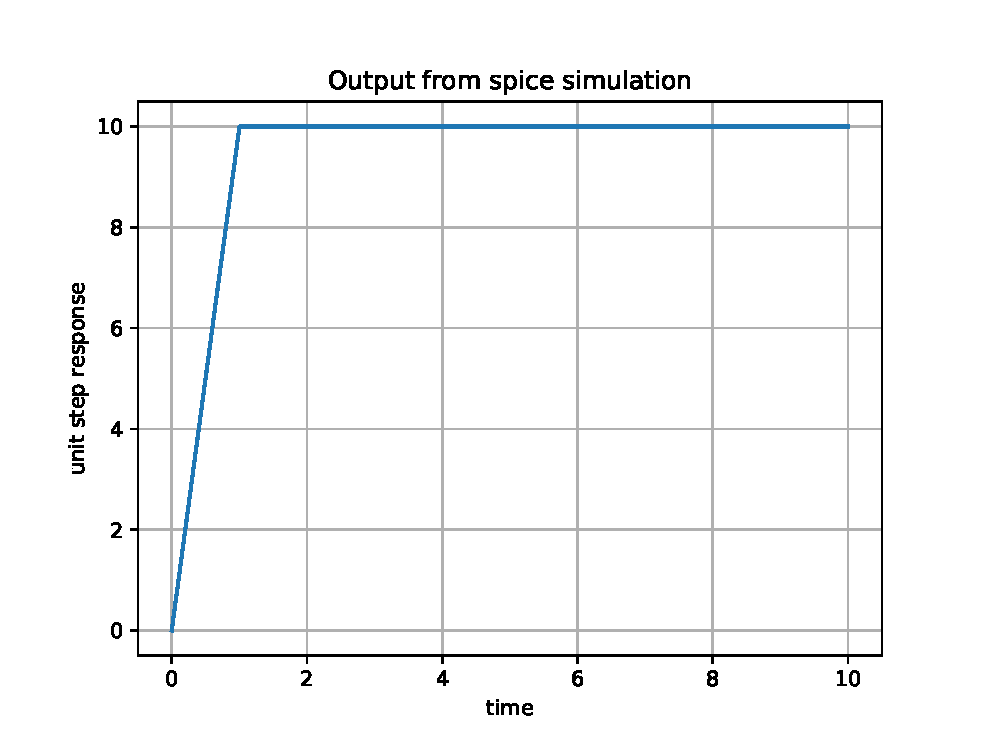
\includegraphics[width=\columnwidth]{./figs/ee18btech11005/ee18btech11005_spice.eps}
\caption{}
\label{fig:ee18btech11005_3}
\end{figure}
\end{enumerate}


